    \begin{figure}[!htbp]
        \centering
        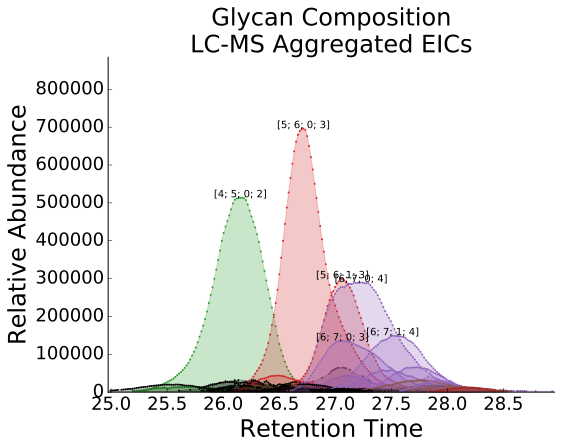
\includegraphics[width=0.45\textwidth,valign=t]{figure/agp_chromatograms.pdf}
        \includegraphics[width=0.45\textwidth,valign=t]{figure/agp_abundances.pdf}
        \caption{\textit{20150930-06-AGP} Glycan Relative Abundances}
        \label{fig:agp_aggregated_eics}
    \end{figure}

    \begin{table}
        \begin{minipage}[t]{0.25\linewidth}
            \vspace{0pt}
            (a)
            \centering
            
    \begin{tabular}{l | c}
        Group & $\tau$ \\
        \hline
        high-mannose & 0.00 \\
        hybrid & 11.81 \\
        bi-antennary & 15.19 \\
        asialo-bi-antennary & 1.28 \\
        tri-antennary & 21.46 \\
        asialo-tri-antennary & 0.98 \\
        tetra-antennary & 14.01 \\
        asialo-tetra-antennary & 0.00 \\
        penta-antennary & 9.61 \\
        asialo-penta-antennary & 0.00 \\
    \end{tabular}
    
            
        \end{minipage}
        \hspace{1cm}
        \begin{minipage}[t]{0.55\linewidth}
            \vspace{0pt}
            (b)
            \centering
            
    \begin{footnotesize}
    \begin{tabular}{l|p{2cm} p{2cm}}
Glycan Compostion &  Unregularized Score &  Regularized Score \\
\hline
\{Hex:5; HexNAc:4; Neu5Ac:1\}        &                13.33 &              10.00 \\
\{Hex:5; HexNAc:4; Neu5Ac:2\}        &                23.36 &              16.47 \\
\{Fuc:1; Hex:5; HexNAc:4; Neu5Ac:2\} &                13.92 &              15.11 \\
\{Hex:6; HexNAc:5; Neu5Ac:2\}        &                19.77 &              17.49 \\
\{Hex:6; HexNAc:5; Neu5Ac:3\}        &                20.13 &              17.60 \\
\{Fuc:1; Hex:6; HexNAc:5; Neu5Ac:2\} &                17.68 &              17.12 \\
\{Fuc:1; Hex:6; HexNAc:5; Neu5Ac:3\} &                17.53 &              17.08 \\
\{Fuc:2; Hex:6; HexNAc:5; Neu5Ac:3\} &                12.97 &              16.40 \\
\{Hex:7; HexNAc:6; Neu5Ac:2\}        &                17.96 &              16.21 \\
\{Hex:7; HexNAc:6; Neu5Ac:3\}        &                17.35 &              16.18 \\
\{Hex:7; HexNAc:6; Neu5Ac:4\}        &                20.81 &              16.55 \\
\{Fuc:1; Hex:7; HexNAc:6; Neu5Ac:2\} &                12.55 &              15.59 \\
\{Fuc:1; Hex:7; HexNAc:6; Neu5Ac:3\} &                17.32 &              15.91 \\
\{Fuc:1; Hex:7; HexNAc:6; Neu5Ac:4\} &                17.17 &              15.95 \\
\{Fuc:2; Hex:7; HexNAc:6; Neu5Ac:3\} &                 8.66 &              14.98 \\
\{Fuc:2; Hex:7; HexNAc:6; Neu5Ac:4\} &                16.66 &              15.61 \\
\{Fuc:3; Hex:7; HexNAc:6; Neu5Ac:4\} &                13.77 &              15.28 \\
\{Hex:8; HexNAc:7; Neu5Ac:3\}        &                13.27 &              12.00 \\
\{Hex:8; HexNAc:7; Neu5Ac:4\}        &                12.81 &              11.97 \\
\{Fuc:1; Hex:8; HexNAc:7; Neu5Ac:3\} &                 8.78 &              11.48 \\
\{Fuc:1; Hex:8; HexNAc:7; Neu5Ac:4\} &                10.66 &              11.62 \\
\{Fuc:2; Hex:8; HexNAc:7; Neu5Ac:4\} &                 9.66 &              11.45 \\
\{Fuc:3; Hex:8; HexNAc:7; Neu5Ac:4\} &                 7.59 &              11.25 \\
\{Hex:9; HexNAc:8; Neu5Ac:4\}        &                11.12 &               9.80 \\
\{Hex:9; HexNAc:8; Neu5Ac:5\}        &                 9.15 &               9.58 \\
\end{tabular}

    \end{footnotesize}
    
        \end{minipage}
        \caption{
                 Search Results for \textit{20150930-06-AGP}.
                 (a) Estimated $\mathbf{\tau}$ for grid with ${\hat \gamma} = 14.837758$.
                 (b) Scores For Identified Glycans of grid with ${\hat \lambda} = 0.99$.}
        \label{tbl:agp_score_table}
    \end{table}
